\section{Data}
This study uses the CAMELS-US dataset (\href{https://doi.org/10.1016/0022-1694(89)90184-4}{https://doi.org/10.1016/0022-1694(89)90184-4}), which provides daily hydro-meteorological time series for minimally disturbed catchments across the contiguous United States\cite{CAMELS}. We select this dataset for three reasons: (1) catchments are weakly affected by direct human regulation, which helps identify more robust hydrological patterns; (2) long and standardized daily forcing--streamflow records support deep learning time-series training and cross-basin comparison\cite{hess-camels}; and (3) the data organization aligns with large-sample hydrology workflows, enabling reproducible evaluation\cite{nearing2021role}. To ensure temporal consistency across stations, we use a common analysis period from 1980-01-01 to 2014-12-31.

Because streamflow record availability varies across stations, we apply a unified quality-control procedure within this period. Stations with more than 100 missing daily values in the target streamflow series are excluded, whereas stations with at most 100 missing days are retained and missing values are filled by linear interpolation. After preprocessing, 521 stations remain for subsequent analysis, as Fig~\ref{fig:station} shows. All retained stations provide multi-year continuous records over the common window (well beyond 20 years), ensuring sufficient sample size for deep learning training.

\begin{figure*}[htbp]
    \centering
    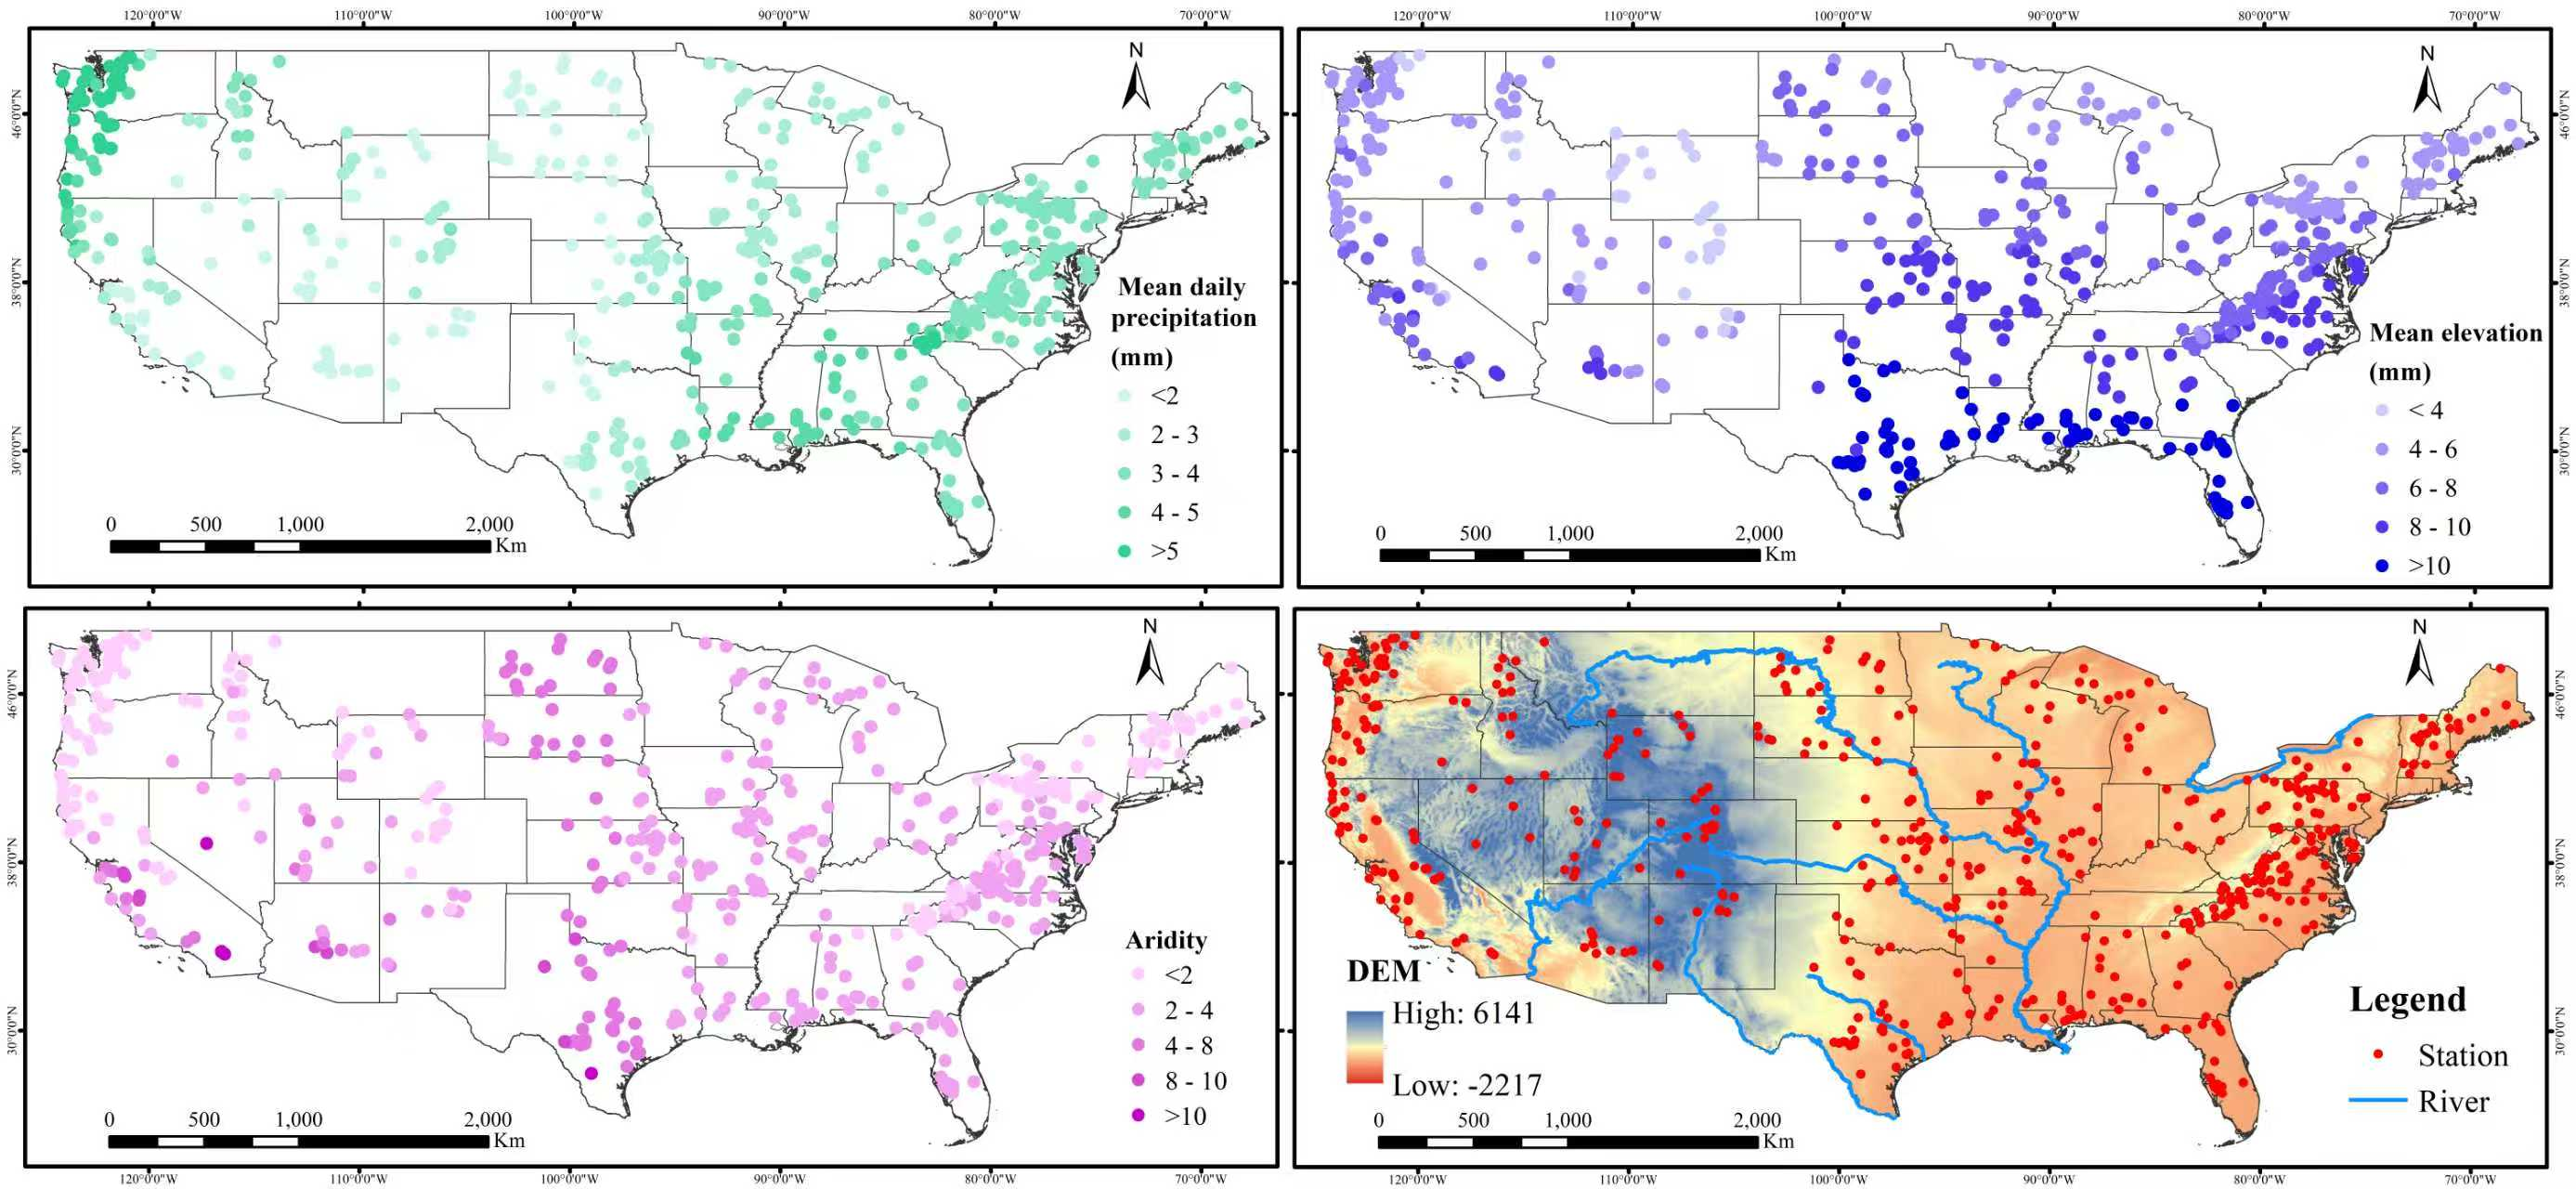
\includegraphics[width=\textwidth]{Figures/MAP.png}
    \caption{
	Spatial distribution of selected streamflow stations after quality control
    }
    \label{fig:station}
\end{figure*}

The model input variables are summarized in Table~\ref{tab:input_features}. For each station, seven daily meteorological forcing variables from Daymet are used, and daily streamflow is additionally incorporated to represent antecedent hydrological state knowledge.

\begin{table}[htbp]
	\centering
	\caption{Selected Input Meteorological and Hydrological Variables}
	\label{tab:input_features}
	\begin{tabular*}{\textwidth}{@{\extracolsep{\fill}}lll}
		\toprule
		Group & Feature name & Unit \\
		\midrule
		\multirow{2}{*}{Energy} & day length (dayl) & s day$^{-1}$ \\
		& shortwave radiation (srad) & W m$^{-2}$ \\
		\multirow{2}{*}{Temperature} & maximum air temperature (tmax) & $^\circ$C \\
		& minimum air temperature (tmin) & $^\circ$C \\
		Atmospheric moisture & water vapour pressure (vp) & Pa \\
		Precipitation & precipitation (prcp) & mm day$^{-1}$ \\
		Snow & snow water equivalent (swe) & mm \\
		Runoff & streamflow (Q) & mm day$^{-1}$ \\
		\bottomrule
	\end{tabular*}
\end{table}

The prediction task is formulated as a sequence-to-one regression problem: a sliding window of length $L=15$ days is used to predict streamflow at the next time step. All features are standardized using training-set statistics. Data are then split chronologically into training (70\%), validation (15\%), and test (15\%) subsets.

The model is implemented in Python 3.10 using PyTorch, and all experiments are conducted on a Linux server equipped with NVIDIA CUDA-enabled GPUs. The three-stage training pipeline (dense pre-training, weight sparsification, and mask learning) uses a single AdamW optimizer with weight decay. Hyperparameters are tuned via Bayesian optimization\cite{BO_OPT}. The search space covers learning rate ($10^{-4}$--$10^{-2}$), batch size (32--256), hidden size (16--256), number of layers (1--16), target weight sparsity (0.7--0.95), target activation sparsity (0.6--0.9), and mask regularization strengths $\lambda_{\mathrm{mask}}$ and $\lambda_{\mathrm{in}}$ ($10^{-5}$--$10^{-3}$). The optimization objective is validation NSE, and the selected configuration is applied consistently across all training stages and downstream explainability analyses. Additional details can be found in Supplementary Notes 2.1.